\section{Families B and C in Full}
\label{app:families}

Table~\ref{tab:drift} gives the median drift at natural boundaries. Family~B
tests the hybrid only; the other two models are shown for reference. At snapped
boundaries drift was exactly zero on Ornith and Qwen3 in every condition.
Table~\ref{tab:contrasts} gives the six contrasts of family~C. C2 and C3 are
numerically identical because snapped drift was exactly zero on both the hybrid
and the dense model, so the interaction reduces to the natural-boundary
difference.

\begin{table}[h]
\caption{Median per-turn mean JSD at natural boundaries, 90 turns per cell
(descriptive; the pre-registered family~B estimate is the mean).}
\label{tab:drift}
\small
\begin{tabular}{@{}lcccc@{}}
\toprule
 & \multicolumn{2}{c}{Short history} & \multicolumn{2}{c}{Long history} \\
Model & explicit & ambiguous & explicit & ambiguous \\
\midrule
Ornith & $\DriftOrnithShortExp$ & $\DriftOrnithShortAmb$ & $\DriftOrnithLongExp$ & $\DriftOrnithLongAmb$ \\
Spark & $\DriftSparkShortExp$ & $\DriftSparkShortAmb$ & $\DriftSparkLongExp$ & $\DriftSparkLongAmb$ \\
Qwen3 & $\DriftQwenShortExp$ & $\DriftQwenShortAmb$ & $\DriftQwenLongExp$ & $\DriftQwenLongAmb$ \\
\bottomrule
\end{tabular}
\end{table}

\begin{table*}[t]
\caption{Family~C: mechanism contrasts (confirmatory). ``More / less'' counts
the turns on which the first side of the contrast was larger or smaller. The
estimate is the mean paired difference in per-turn mean JSD, except for C6,
which is a difference in action-change rate in percentage points. Intervals are 95\% paired
bootstrap intervals.}
\label{tab:contrasts}
% src for the Pairs and Claimed columns: docs/findings/2026-09-11-main-study.md, "Family C"
\small
\begin{tabular}{@{}llrrrll@{}}
\toprule
 & Contrast & Pairs & More & Less & Estimate and 95\% interval & Claimed \\
\midrule
C1 & Snapping on the hybrid (natural $-$ snapped) & 360 & \COnePos & \COneNeg & $\COneEst$ \ $[\COneLo,\ \COneHi]$ & yes \\
C2 & Snapping $\times$ architecture (hybrid vs.\ dense) & 360 & \CTwoPos & \CTwoNeg & $\CTwoEst$ \ $[\CTwoLo,\ \CTwoHi]$ & no \\
C3 & Hybrid $-$ dense, natural boundary & 360 & \CThreePos & \CThreeNeg & $\CThreeEst$ \ $[\CThreeLo,\ \CThreeHi]$ & no \\
C4 & Hybrid $-$ sliding window, natural boundary & 360 & \CFourPos & \CFourNeg & $\CFourEst$ \ $[\CFourLo,\ \CFourHi]$ & yes \\
C5 & Long $-$ short history on the hybrid & 180 & \CFivePos & \CFiveNeg & $\CFiveEst$ \ $[\CFiveLo,\ \CFiveHi]$ & no \\
C6 & Ambiguous $-$ explicit on the hybrid (action change) & 180 & \CSixPos & \CSixNeg & \CSixEstPct{} \ [\CSixLoPct,\ \CSixHiPct] points & yes \\
\bottomrule
\end{tabular}
\end{table*}

\section{Per-Turn Drift}
\label{app:drift}

Figure~\ref{fig:drift} shows the drift of every natural-boundary turn.

\begin{figure}[h]
\centering
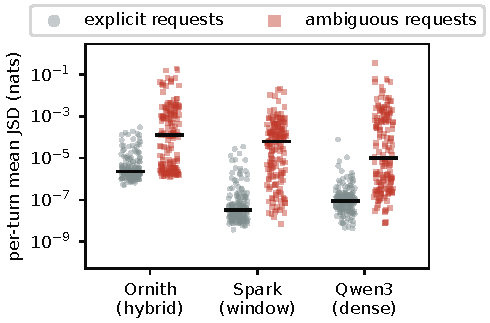
\includegraphics[width=\columnwidth]{figures/drift_per_turn.pdf}
\caption{Per-turn mean JSD between restore and recompute at natural
boundaries, one point per turn, both history lengths. Black bars are
medians pooled over both history lengths (descriptive). Ornith is the hybrid recurrent model, Spark the sliding-window model,
Qwen3 the dense model.}
\label{fig:drift}
\end{figure}

\section{Sliding-Window Follow-Up}
\label{app:spark}

This follow-up is exploratory. Its plan and predictions were committed before
it ran, but it was not part of the pre-registration, and it uses one prompt:
the first long-history main-study turn, 4{,}268 tokens, with 13 reuse
boundaries and 16 generated tokens per case. Table~\ref{tab:sparkgrid} shows
which restores were bit-exact. With default settings, the rule ``exact when
$k$ is a multiple of \nub{} and $k \leq 512$'' fits all \SparkCases{} cases.
The alternatives fit worse: ``aligned and $k \leq \nub$'' fails twice,
``$k \leq 512$ regardless of alignment'' six times, and alignment alone 20
times. In a fifth run without \texttt{-{}-swa-full}, the server saved each slot
correctly but then evaluated the whole prompt on all 13 restores, so no restore
was proven and every output equalled recompute.

\begin{table}[h]
\caption{Spark: bit-exact (E) or inexact (--) restores by reuse boundary $k$
and server configuration (exploratory). FA off: flash attention disabled.}
\label{tab:sparkgrid}
% src: docs/findings/2026-09-11-spark-window.md, "Exact grid"
\small
\begin{tabular}{@{}rcccc@{}}
\toprule
 & \multicolumn{3}{c}{\nub{} (default settings)} & FA off \\
$k$ & 256 & 512 & 1{,}024 & 512 \\
\midrule
256 & E & -- & -- & -- \\
384 & -- & -- & -- & -- \\
512 & E & E & -- & E \\
640 & -- & -- & -- & -- \\
768 & -- & -- & -- & -- \\
1{,}024 & -- & -- & -- & E \\
1{,}280 & -- & -- & -- & -- \\
1{,}536 & -- & -- & -- & E \\
2{,}048 & -- & -- & -- & E \\
2{,}560 & -- & -- & -- & E \\
3{,}072 & -- & -- & -- & -- \\
3{,}584 & -- & -- & -- & -- \\
4{,}096 & -- & -- & -- & -- \\
\bottomrule
\end{tabular}
\end{table}

\section{Changed Actions}
\label{app:examples}

% src: docs/findings/study/changed_turns.json; probabilities from data/study/*.jsonl (replicate 1, top-10 log-probabilities)
Table~\ref{tab:examples} shows three changed turns side by side, all on Ornith
at natural boundaries, and Table~\ref{tab:census} lists all \ChangesTotal{}.
Decoding is greedy, so each arm emits its more probable token, and every change
reproduced in both replicates. The two request types that ask the model to
choose between tools produced no changes.

\begin{table*}[p]
\caption{Three changed turns on Ornith at natural boundaries. ``At
token'' gives the two most probable tokens, with probabilities in
percent, at the first generated position where the arms differ; \textsc{call}
is the token that opens a tool call. Values in bold are where the outputs
part.}
\label{tab:examples}
\small
\begin{tabular}{@{}>{\raggedright\arraybackslash}p{0.15\textwidth}>{\raggedright\arraybackslash}p{0.39\textwidth}>{\raggedright\arraybackslash}p{0.39\textwidth}@{}}
\toprule
 & Recompute & Restore \\
\midrule
\multicolumn{3}{@{}l}{\textit{(a) Long history, ``Pull up that record again'', $k=6{,}416$, action margin 0.09}} \\
At token 0 & \textbf{\textsc{call} 41.0}, `The' 37.4 & \textbf{`The' 53.3}, \textsc{call} 40.3 \\
Output & calls \texttt{lookup\_record(73)} & ``The record you're referring to is record 73, which has field=beta value=701.'' \\
\midrule
\multicolumn{3}{@{}l}{\textit{(b) Short history, ``Write that up for me'', $k=1{,}212$, action margin 0.61}} \\
At token 0 & \textbf{`I' 44.6}, \textsc{call} 24.2 & \textbf{\textsc{call} 34.0}, another token 28.8 \\
Output & ``I'm not sure which task or information you're referring to. Could you clarify what you'd like me to write up?'' & calls \texttt{format\_report} with the title ``Record Lookup Summary'' and three records from the history \\
\midrule
\multicolumn{3}{@{}l}{\textit{(c) Long history, ``Add up the numbers from earlier'', $k=6{,}351$, action margin 0.22}} \\
At token 38 & \textbf{`6' 55.4}, `9' 44.4 & \textbf{`9' 65.4}, `6' 34.3 \\
Output & \texttt{compute\_sum([68, 110, 72, 118, 36, \textbf{65}, 90, \ldots, 74])}, 23 values & \texttt{compute\_sum([68, 110, 72, 118, 36, \textbf{90}, \ldots, 74])}, 22 values; 65 is missing \\
\bottomrule
\end{tabular}

\bigskip
\caption{All \ChangesTotal{} changed actions. History: prefix band. Request:
``Add up the numbers from earlier'', ``Pull up that record again'' or ``Write
that up for me''. $k$: reuse boundary. Pos.: first generated position where
the arms differ. The two token columns give the two most probable tokens there,
with probabilities in percent; \textsc{call} opens a tool call and
\textit{other} is a token that neither arm emitted. Arguments: the same tool
with different arguments. The three snapped rows are Spark at
$k=4{,}096$, where snapping is not exact (\S\ref{sec:mechanism}). Turn
identifiers and full outputs are in the repository.}
\label{tab:census}
\footnotesize
\setlength{\tabcolsep}{4pt}
\begin{tabular}{@{}llllrrrlll@{}}
\toprule
Model & History & Request & Boundary & $k$ & Margin & Pos. & Recompute top two & Restore top two & Change \\
\midrule
Ornith & long & Add up & natural & 6{,}387 & 0.07 & 29 & `7' 35.6, `2' 33.4 & `2' 46.9, `9' 31.5 & arguments \\
Ornith & long & Record & natural & 6{,}388 & 1.44 & 0 & \textsc{call} 76.9, \textit{other} 18.1 & `I' 37.9, \textit{other} 32.6 & tool$\to$text \\
Ornith & long & Add up & natural & 6{,}467 & 0.21 & 16 & `6' 53.6, `2' 42.4 & `2' 60.4, `6' 34.2 & tool$\to$text \\
Ornith & long & Record & natural & 6{,}294 & 0.13 & 0 & \textsc{call} 45.3, `The' 39.6 & `The' 63.1, \textsc{call} 22.8 & tool$\to$text \\
Ornith & long & Add up & natural & 6{,}420 & 0.03 & 55 & `9' 58.2, `3' 41.0 & `3' 53.0, `9' 46.3 & arguments \\
Ornith & long & Add up & natural & 6{,}482 & 0.03 & 30 & `5' 55.0, `6' 45.0 & `6' 50.8, `5' 49.2 & arguments \\
Ornith & long & Add up & natural & 6{,}506 & $<$0.01 & 16 & `6' 46.3, `2' 45.9 & `2' 65.9, `6' 24.5 & arguments \\
Ornith & long & Record & natural & 6{,}416 & 0.09 & 0 & \textsc{call} 41.0, `The' 37.4 & `The' 53.3, \textsc{call} 40.3 & tool$\to$text \\
Ornith & long & Add up & natural & 6{,}515 & 0.06 & 130 & `8' 46.2, `4' 43.4 & `4' 45.9, `8' 44.2 & arguments \\
Ornith & long & Add up & natural & 6{,}351 & 0.22 & 38 & `6' 55.4, `9' 44.4 & `9' 65.4, `6' 34.3 & arguments \\
Ornith & long & Add up & natural & 6{,}384 & $<$0.01 & 33 & `4' 59.9, `1' 36.7 & `1' 49.0, `4' 48.0 & arguments \\
Ornith & short & Write up & natural & 1{,}212 & 0.61 & 0 & `I' 44.6, \textsc{call} 24.2 & \textsc{call} 34.0, \textit{other} 28.8 & text$\to$tool \\
Ornith & short & Add up & natural & 1{,}233 & 0.46 & 16 & `4' 61.0, `9' 38.5 & `9' 64.8, `4' 34.7 & arguments \\
Ornith & short & Record & natural & 1{,}242 & 0.19 & 17 & `1' 54.5, `7' 45.1 & `7' 52.7, `1' 46.9 & arguments \\
Spark & long & Add up & natural & 4{,}300 & 0.14 & 0 & `The' 31.7, \textsc{call} 27.7 & \textsc{call} 34.6, `The' 31.8 & text$\to$tool \\
Spark & long & Add up & snapped & 4{,}096 & 0.11 & 0 & `The' 30.9, \textsc{call} 27.6 & \textsc{call} 32.0, `The' 22.6 & text$\to$tool \\
Spark & long & Add up & snapped & 4{,}096 & 0.11 & 0 & `The' 36.4, \textsc{call} 32.6 & \textsc{call} 31.7, `The' 28.8 & text$\to$tool \\
Spark & long & Add up & natural & 4{,}383 & 0.14 & 0 & `The' 24.7, \textit{other} 21.4 & \textsc{call} 30.5, `The' 20.3 & text$\to$tool \\
Spark & long & Add up & snapped & 4{,}096 & 0.14 & 0 & `The' 24.7, \textit{other} 21.4 & \textsc{call} 35.3, `The' 17.5 & text$\to$tool \\
Spark & long & Record & natural & 4{,}264 & 0.31 & 0 & \textsc{call} 47.5, `The' 34.7 & `The' 43.1, \textsc{call} 36.0 & tool$\to$text \\
Spark & long & Add up & natural & 4{,}242 & 0.64 & 0 & `The' 31.9, \textit{other} 16.8 & \textsc{call} 28.0, `The' 23.9 & text$\to$tool \\
Spark & short & Record & natural & 773 & 0.05 & 10 & `3' 51.2, `4' 48.8 & `4' 61.4, `3' 38.6 & arguments \\
Spark & short & Add up & natural & 782 & 0.15 & 0 & \textsc{call} 43.8, `The' 37.9 & `The' 39.9, \textsc{call} 30.3 & tool$\to$text \\
Qwen3 & long & Write up & natural & 5{,}340 & 3.09 & 0 & `The' 87.0, \textsc{call} 4.0 & \textsc{call} 32.3, \textit{other} 26.3 & text$\to$tool \\
Qwen3 & long & Record & natural & 5{,}296 & 1.25 & 0 & \textsc{call} 72.9, `I' 21.0 & `I' 43.2, \textsc{call} 41.1 & tool$\to$text \\
Qwen3 & long & Record & natural & 5{,}265 & 0.13 & 0 & \textsc{call} 45.7, `I' 40.2 & `I' 62.3, \textit{other} 23.2 & tool$\to$text \\
Qwen3 & short & Add up & natural & 958 & 0.17 & 0 & `I' 50.1, `The' 42.4 & `The' 67.9, `I' 21.2 & text$\to$tool \\
Qwen3 & short & Add up & natural & 936 & 1.52 & 23 & `]' 87.5, `,' 12.5 & `,' 94.3, `]' 5.7 & arguments \\
Qwen3 & short & Add up & natural & 963 & 0.48 & 0 & \textsc{call} 47.0, `The' 29.1 & `The' 40.7, \textit{other} 34.0 & tool$\to$text \\
Qwen3 & short & Add up & natural & 965 & 0.20 & 0 & `The' 54.5, `I' 44.5 & `I' 56.6, `The' 42.0 & tool$\to$text \\
\bottomrule
\end{tabular}
\end{table*}

\section{Measurement Safeguards}
\label{app:safeguards}

% src: README.md, "How the measurement is kept honest"; docs/findings/2026-09-10-g2.md; docs/findings/2026-09-10-g3.md
\begin{itemize}
\item \textbf{Prompt rendering.} The server's template endpoint does not accept
  tool schemas, so prompts are rendered offline from each model's embedded chat
  template. The offline rendering was checked against the server: byte for byte
  without tools, and token count for token count with tools.
\item \textbf{Tool-call parsing.} Each model has its own tool-call syntax. A
  parsed call is accepted only if writing it back through the model's chat
  template reproduces the model's exact text. All 161 parsed calls in the
  validation set did.
\item \textbf{Blinding.} The runner printed only arm-validity counts while the
  study ran, wrote whole turns atomically, and refused a server with a different
  build or model. The analysis script refused to run until all three models had
  finished.
\item \textbf{Gates.} Four gate experiments preceded the study: G0 (the state
  interface works), G1 (the mechanism, \S\ref{sec:mechanism}), G2 (rendering and
  parsing) and G3, a pilot on 20 separate turns per model that checked the arm
  proofs, the exactness of snapped restores on short histories, and that the
  hybrid drifted at natural boundaries. Pilot turns are not in the analysis.
\item \textbf{Tests.} The harness has a test suite that needs no GPU, including
  a simulated server in which micro-batch tiling is the only source of
  divergence.
\end{itemize}

\section{A Side Finding: Tool-Call Grammar}
\label{app:grammar}

% src: docs/findings/2026-09-11-spark-argument-order.md
This observation is exploratory and concerns one conversation.
While validating the parsers we saw one Spark tool call whose arguments
differed between our parse and the server's. We first attributed this to the
server's parser. Reproducing it inside llama.cpp showed the parser was correct:
the server's tool-call grammar for Spark's format requires the required
arguments in schema order, Spark prefers a different order, and under the
grammar it wrote a different argument value. Reversing only the order of the
schema's properties restored the model's unconstrained output. An open pull
request makes the argument order free~\cite{llamacpp-26472}; while testing it
we reported, on its thread, a regression for the Laguna-XS templates. The main study
generates without a tool grammar and is not affected.

\section{Reproduction}
\label{app:repro}

Code, raw gate reports, the per-turn analysis table and all changed turns are
at \url{https://github.com/manuelgamal/driftmatrix}. The analysis plan is
frozen at the Git tag named \texttt{prereg-2026-09-10}.
The test suite needs no GPU. With a
model file and a llama.cpp build:

{\footnotesize
\begin{verbatim}
llama-server -m <model.gguf> --jinja -c 8192 -ngl 99
  -np 1 -b 2048 -ub 512 --cache-ram 0
  --ctx-checkpoints 0 --slot-save-path <dir>
  --port 8090     # add --swa-full for Spark
python scripts/run_study.py --model ornith
  --gguf <model.gguf> --slot-dir <dir>
python scripts/analyze_study.py --gguf ornith=<..>
  --gguf qwen3=<..> --gguf spark=<..>
python scripts/make_figures.py --paper
python scripts/paper_numbers.py
\end{verbatim}
}
